\section{Introduction}

Recent years have witnessed widespread use of sophisticated frameworks such as Hadoop\cite{hadoop}, Spark\cite{spark} and Apache Tez\cite{tez}.
Tremendous effeots have been paid to improve the speed and of large-scale dataparallel systems computing process, from the the low level storage system to scheduling algorithms.

% take over shuffle
%shuffle characteristic
Although highly optimized, DAG computing framworks are derived from MapReduce\cite{mapreduce}, contains a hard barrier between computing stages. The terminology of this barrier is Shuffle. Shuffle contains two parts on the connecting stages. On the side of ancestor stage, shuffle is resoponsible for writing intermediate result to disk. On the side of successor stage, shuffle fetches intermediate result from remote disks in cluster. This shuffle process introduces frequent I/O operations,
% design inconsistent
 which result in a significiant performance and cluster utilization decline. For instance, a MapReduce trace analysis from Facebook shows that shuffle accounts for 33\% JCT on average, up to 70\% in shuffle-heavy jobs\cite{manage}.

% shuffle operations

% three resource coordinate 不好
% 计算和I/O couple, why
% why disk, reason!!!, 不重视
% common problems
The straight forward way is to start reduce tasks earlier. Apache Hadoop\cite{hadoop} provides a mechanism, which schedules reduce tasks when a certain portion of map tasks completed. So that the shuffle delay can be mitigated by overlapping execution of reduce phase and map phase. Other publications also purpose solutions to pre-schedule reduce tasks\cite{ihadoop, ishuffle, dynmr}. However this early scheduling of reduce tasks occupies new task slots, which degrades system performance. We argue that current DAG frameworks are under utilized due to coarse granularity of resources allocation. Nearly all
MapReduce based task scheduling algorithms use time slotted model. Specifically, when a task is launched, the framework offers it a bundle of resources (i.e. CPU and memory), which are dedicated to this task during the time in its "slot". As shown in the upper part of Figure \ref{fig:workflow}, this "slot" can be released until the map tasks finish "Shuffle Write" on disk. And the "slot" is occupied when the of reduce tasks begin to read shuffle data from remote nodes through network, which is presented as "Shuffle Read". As depicted in Figure \ref{fig:workflow}, the hardware resources in a slot are under utilized in those two I/O intensive phases. To this end, we proposed a quetion, \textit{can we efficiently optimize shuffle without manually change every DAG framework?} 

\begin{figure}
	\centering
	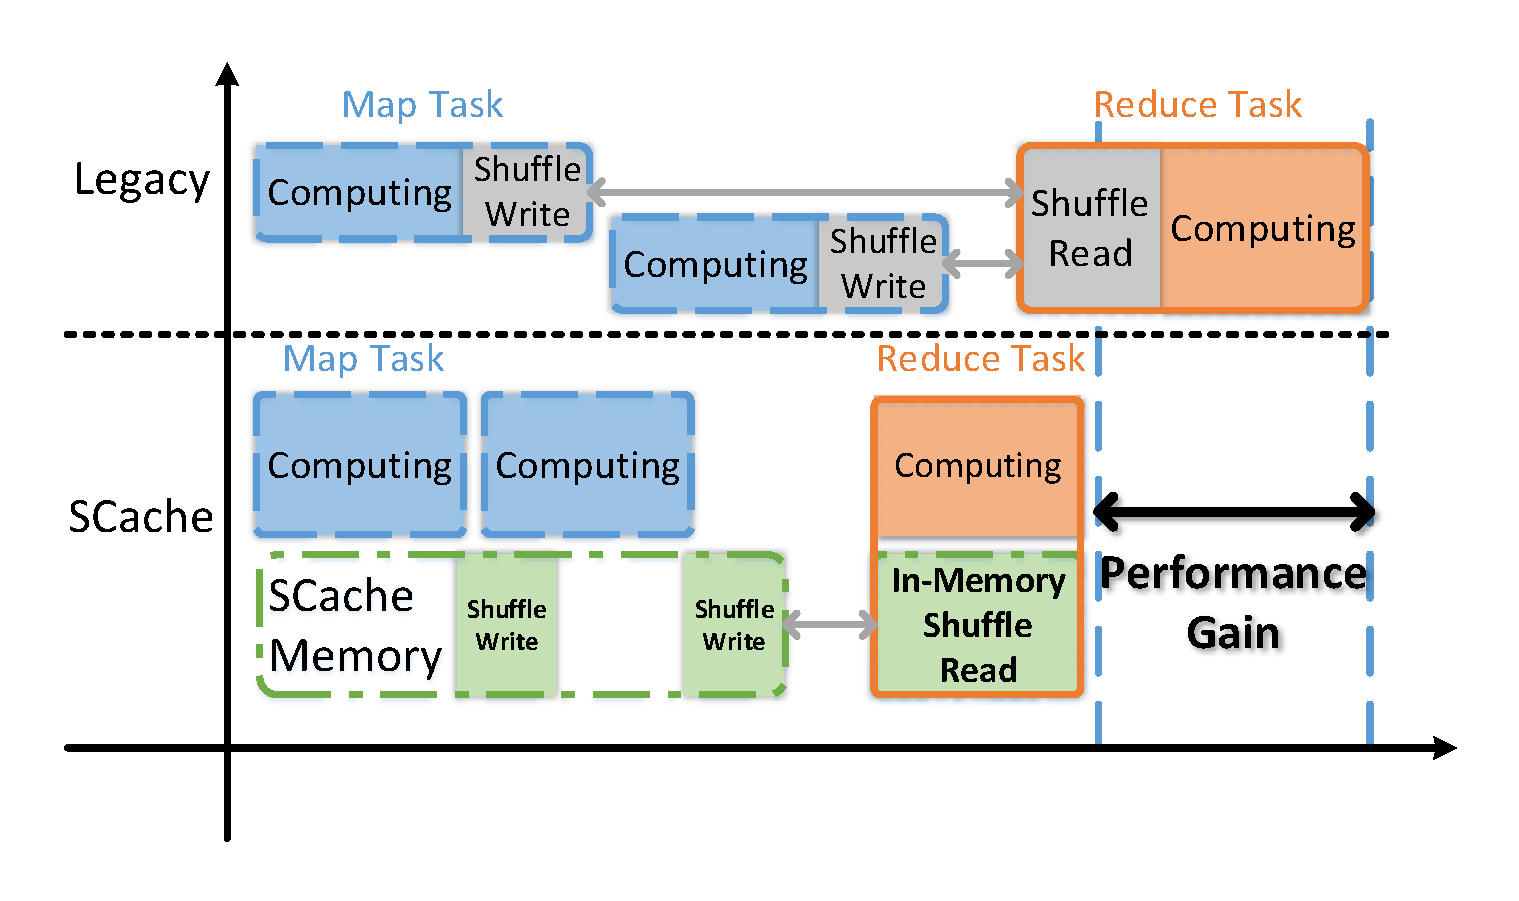
\includegraphics[width=\linewidth]{fig/workflow}
	\caption{Workflow Comparison between Legacy DAG Computing Frameworks and Frameworks with SCache}
	\label{fig:workflow}
\end{figure}


% 针对性的提出这三个点
% three resource coordinate 不好
% 计算和I/O couple, why
% why disk, reason, 不重视
% common problems
% 总起:普适性工具
% pre-fetch but not pre-execute
% byproduct: more balance
% memory instead of disk

% challenge point by point, inside the problem

In this paper, we introduce SCache, an plugin system to remove shuffle latency without occupying slot. The workflow of DAG computing with SCache is presented in Figure \ref{fig:workflow}. By decoupling shuffle from computing, pre-scheduling tasks and pre-fetching shuffle data for DAG computing frameworks, the shuffle latency can be mitigated with no degradation on the DAG framework. In Figure \ref{fig:workflow}, SCache hijacks the intermediate data of a map task from memory space of the slot. The disk operation is skipped and the intermediate data is immediately shuffled through network to the pre-assigned remote node for further reduce tasks execution. By optimizing the disk operation and starting the network transfer ahead of reduce tasks, SCache can help the DAG framework achieve a significant performance gain.

The main challenge to achieve this optimization is \textit{pre-scheduling reduce tasks}. The challenge is not critical for the simple DAG computing such as Hadoop MapReduce\cite{mapreduce}. Unfortunately the complexity of DAG can amplify the defects of na\"{i}ve pre-scheduling schemes. In particular, randomly assign reduce tasks to nodes can result in a collision of two heavy tasks on a same node. This collision can aggravate data skew and hurts the performance of the DAG frameworks. To address this challenge, we propose a heuristic scheme to predict the shuffle output distribution and schedule reduce tasks.

The second challenge is the \textit{limitation of memory space}. To prevent shuffle data touching the disk, SCache leverages extra memory to store the shuffle data. However, the memory is a precious resource for DAG computing, especially for in-memory framework such as Spark\cite{spark}. In order to optimize shuffle without hurting the performance of DAG frameworks, SCache only reserves small fraction of memory to store shuffle data. To maximum the performance gain of optimization and memory utilization, we propose two constraints: all-or-nothing and context-aware. The memory management scheme follows these two contraints to switch shuffle data blocks on and off reserved memory.

We implement SCache and a daemon in Apache Spark\cite{apachespark}. Our evaluation in a 50-node Aamazon EC2 cluster. We conduct basic test like GroupByTest.We also evaluate benchmark like Terasort\cite{spark-tera} and standard workloads like TPC-DS\cite{tpcds} for multi-tenant modeling. In a nutshell, SCache can eliminate explict shuffle process by at most 88\% in varied application scenarios.




